\chapter{System Design and Architecture}
\label{ch:design}
\section{Requirements Analysis}
CAM-F's design emerged from systematic analysis of film production constraints, technical requirements and user needs. Rather than pursuing technical sophistication for its own sake, every design decision prioritised practical deployability and operational simplicity whilst maintaining the modularity needed for research advancement. Through extensive literature review of industry workflows, analysis of existing professional production tools, and investigation of documented continuity practices in film, we identified critical requirements that shaped the architectural decisions.
\subsection{Production Environment Constraints}
Film sets present unique deployment challenges absent from typical video-capture software environments. Keeping footage secure and unreleased before official distribution is essential for productions to maintain commercial value. Systems must operate fully offline to ensure full safety whilst maintaining functionality. This might eventually limit the capabilities of specialised detectors that could need access to external tools. However, the project's goals necessitate network isolation, which ensures deployment-ready application and, at the same time, showcases feasibility even in these limited conditions. 
Productions cannot dedicate high-end servers to continuity detection. The system must run on script supervisors' portable hardware that travels between locations and allows for minimal setup costs. Operational simplicity is another key aspect of design requirements. Set personnel focus on filmmaking, not IT administration. Complex deployment procedures or ongoing maintenance requirements would prevent seamless integration into existing workflows. With hundreds of crew members depending on production and tight schedules, reliability of the system is essential. Failures cannot interrupt filming, so graceful degradation takes priority over feature completeness.
\subsection{Performance Requirements}
Temporal analysis of production workflows shows specific performance targets. Reset windows between takes define maximum acceptable processing time. It varies enormously based on shot complexity, crew size, equipment requirements, location constraints and directorial style. Nevertheless, we can estimate the average distribution:
68\% of resets: 2–5 minutes
24\% of resets: 5–15 minutes
8\% of resets: >15 minutes
To capture the majority of opportunities to prevent any anomaly, processing must complete within 5 minutes after the take's cut. For example, given average take lengths of 45 seconds, this requires processing 45 seconds of footage within 345 seconds (including the take length), or 7.6× real-time minimum. This makes time to detect the essential metric requirement for the system.
Another essential requirement is the detection accuracy, which determines the system's trustworthiness and practical potential. Unfortunately, due to the lack of published studies and error rate statistics it is hard to set a distinctive benchmarking for accuracy. Based on vigilance task research demonstrating 10-30\% performance degradation in sustained attention tasks [9], we conservatively estimate human detection accuracy at 75-80\% over typical 10-14 hour production days, accounting for the mitigating effects of professional tools and techniques employed by script supervisors. This provides a baseline against which automated detection performance can be measured.
Important to note that missing a continuity anomaly that reaches final edit proves far more expensive than investigating a false alarm during principal photography. Which makes the false negatives (missed errors) far more relevant than false positives (incorrect alerts).
\subsection{Other Non-Quantifiable Requirements}
Detector extensibility: Different productions face varying continuity challenges. Since covering everything is not feasible, the framework must support development of specialised detectors addressing different error types, from simple prop tracking to complex semantic analysis, without requiring core system modifications.
Result transparency: Detection outputs must provide clear explanations and visual evidence for flagged issues. Script supervisors need to quickly understand why the system flagged a potential error and make informed decisions about its validity.
Workflow integration: The system must integrate seamlessly with existing production practices without disrupting established routines. Script supervisors should access detection results through familiar interfaces that complement, rather than replace, current tools.
Long-term data management: Extended productions accumulate thousands of takes across multiple shooting days. The system must store all captured frames, detection results and associated notes in an organised, searchable structure that enables rapid retrieval of any historical reference. 
\section{Architecture Overview}
CAM-F implements a hybrid architecture combining a monolithic backend with process-isolated detector plugins. The system consists of four primary components: a single Python process hosting all core services, a Tauri-wrapped React frontend, isolated detector processes managed through multiprocessing, and a hierarchical storage system mapped to film production workflows.
Figure 3.1 illustrates the system architecture. The backend process contains Storage, Capture, Detector Framework, and Export services running in shared memory. These services communicate through direct method calls, eliminating serialisation overhead. The API Gateway runs in a separate thread within the same process, providing REST endpoints and SSE (Server-Sent Events) channels for frontend communication. Each detector executes in a sandboxed subprocess with enforced resource limits and restricted filesystem access.

\begin{figure}[h]
\centering
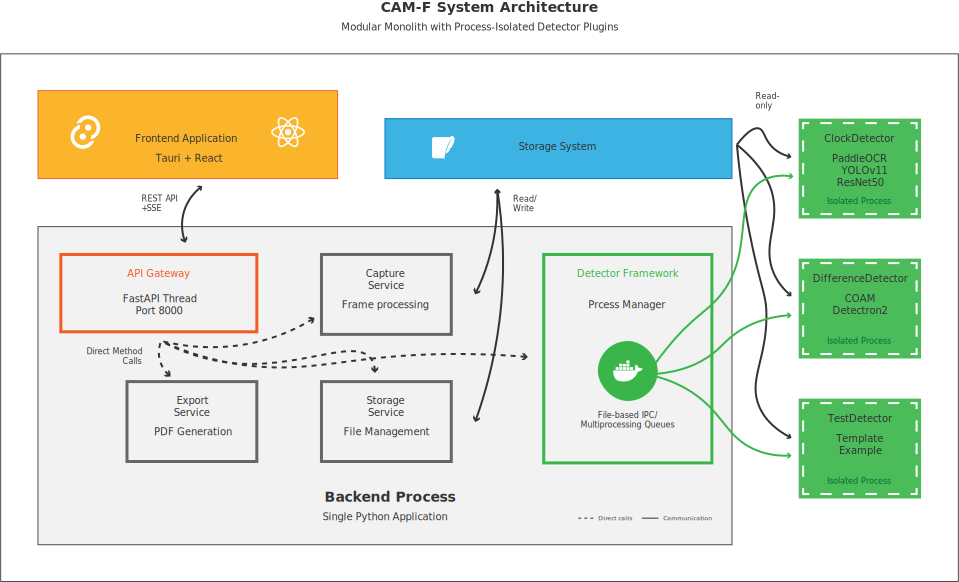
\includegraphics[width=0.9\textwidth]{figures/Architecture.png}
\caption{CAM-F System Architecture showing monolithic backend with sandboxed detector plugins. Services communicate via direct method calls while detectors use JSON-RPC over stdin/stdout.}
\label{fig:architecture}
\end{figure}
\section{Key Design Decisions}
\subsection{Implementation Platforms}
Python serves as CAM-F's backend language due to its dominance in computer vision deployment. All major object detection frameworks, including YOLOv11 and Detectron2 used in our detector implementations, provide Python APIs exclusively. OpenCV's Python bindings enable efficient frame capture and preprocessing without performance penalties through optimised C++ implementations underneath. The multiprocessing module provides process isolation primitives essential for detector sandboxing, handling IPC and lifecycle management through platform-agnostic abstractions.
React powers the frontend to handle real-time UI updates from continuous frame capture. Its virtual DOM (Document Object Model) reconciliation minimises rendering overhead when updating frame previews, helpful for resource-constrained laptops common on film sets. Zustand manages application state with small footprint, whilst TanStack Query handles API communication with built-in retry logic and request deduplication. This technology stack prioritises ecosystem compatibility and production deployment requirements over theoretical performance optimisations, ensuring CAM-F integrates with existing computer vision research whilst remaining deployable by non-technical users.
\subsection{Technology Stack}
FastAPI: The backend uses FastAPI to handle REST endpoints and SSE channels. FastAPI's asynchronous request handling enables concurrent processing of capture commands, storage queries and detector status updates without blocking. Built-in error recovery middleware ensures graceful handling of detector failures without affecting other system components. We also use the framework's automatic OpenAPI schema to generate interactive documentation. It allows developers to test endpoints directly, which supports community-driven development.
Docker SDK: Each detector execution is managed in its own isolated container. When a detector processes frames, the framework spawns a container with comprehensive security controls:
Flexible resource allocation: No default limits on memory, CPU or processes allowing intensive CV/ML workloads to utilise available resources (configurable). 
Filesystem isolation: Read-only root filesystem with writable workspace areas for computation
Network isolation: Disabled networking prevents footage exfiltration
System call filtering: Custom \verb|seccomp| profiles restrict dangerous operations
AppArmor integration: Additional MAC (Mandatory Access Control) layer when available
The SDK's Python interface enables programmatic container lifecycle management, from image building during detector installation to automatic cleanup after processing completion. It is not only essential for safety measures, but also to allow detectors the freedom and control over the environments they need to set up for computation.
SQLite: The storage service uses SQLite as an embedded database for metadata management. ACID-compliant transactions ensure data integrity during unexpected shutdowns. The data model directly maps to production hierarchy: projects, scenes, angles, takes, and frames.
Tauri: The frontend wraps React using Tauri 1.5, which currently only supports native desktop applications for Windows, but can be easily extended to other OS. Tauri produces much smaller executables than similar technologies by leveraging system WebView components rather than bundling browser engines. The framework's secure IPC bridge also contributes to security measures by restricting filesystem access to designated directories.
Server-Sent Events (SSE): Real-time updates flow from backend to frontend through SSE channels. The unidirectional nature matches CAM-F's communication pattern where the server broadcasts capture progress and detector results. SSE's automatic reconnection with exponential backoff handles any interruptions. Event queues limited to 100 messages prevent memory exhaustion whilst maintaining UI responsiveness.
\subsection{Storage Strategy}
The storage architecture mirrors the production hierarchy. CAM-F organises footage by project, scene, angle, and take as shown in Figure 3.2.

\begin{figure}[h]
\centering
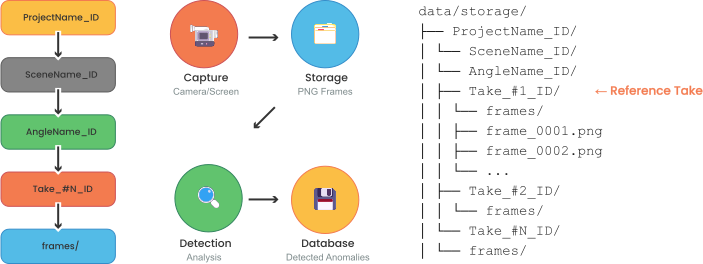
\includegraphics[width=0.7\textwidth]{figures/storage.png}
\caption{Hierarchical storage structure mirroring film production workflow. Each level maps to production concepts with unique IDs preventing naming conflicts.}
\label{fig:storage}
\end{figure}

Individual frames are stored as PNG files enabling random access for detector processing. Scene and custom detector configurations attach at the scene level, as it's being initialised, and are applied across all its descendants. We also automatically establish reference take as baseline for continuity. The first take of each angle automatically becomes the reference unless manually overridden. Subsequent takes compare against this reference for anomaly detection.
Continuity errors detected by the framework are stored in the database where they can be quickly searched and filtered. The system tracks individual detections on each frame (confidence scores, locations, which detector found them), false positives marked by the production team and errors that span multiple frames. Custom result deduplication algorithm prevents alert fatigue from continuous errors. The system groups spatially and temporally proximate detections, presenting them as single issues rather than flooding supervisors with redundant notifications.
\section{Core Framework Components}
\subsection{Real-time Monitoring Pipeline}
The monitoring pipeline implements push-based stream processing, a fundamental design choice that influences the entire system architecture. When the capture service acquires a frame, it immediately pushes the data through the processing pipeline rather than allowing detectors to pull frames on demand. This approach optimises for minimal latency over maximum throughput, reflecting production requirements where immediate feedback proves more valuable than processing efficiency.
Frame data flows through the system using storage as the communication medium rather than memory or network transfer. The capture service writes each frame once to persistent storage, after which multiple detectors read the frame data independently. This pattern appears inefficient compared to in-memory passing, yet provides several critical advantages:
Single source of truth: Frame data exists in one authoritative location
Natural audit trail: All captured frames remain available for review
Reduced memory pressure: No frame duplication across process boundaries
Simplified recovery: System restart automatically recovers all persisted frames
The pipeline adopts a shared-nothing architecture where each detector processes frames independently without inter-detector communication or shared state. This design eliminates coordination overhead and prevents cascading failures, though it prevents any collaborative detection strategies where multiple detectors might share intermediate results. The simplicity and reliability benefits outweigh the potential advantages of multi-detector cooperation.
\subsection{Frontend Event Distribution}
The event system uses SSE for unidirectional server-to-client communication. This design ensures the backend remains the sole authority for state changes. Clients request modifications through REST APIs but cannot directly alter system state, preventing synchronisation conflicts common in bidirectional systems. Events transmit complete state rather than change notifications. Network interruptions become trivial to handle as reconnecting clients receive current state immediately. Internal service communication differs fundamentally from external UI updates. Backend services communicate through direct method calls, ensuring reliable and ordered message delivery. UI clients receive events through SSE with best-effort delivery. When clients fall behind, the system drops older events to maintain real-time relevance. This separation provides appropriate guarantees for each communication type without unnecessary complexity.
The architecture remains deliberately simple. Rather than implementing complex event sourcing or message queuing systems, CAM-F uses straightforward patterns. Multiple clients can subscribe to event streams without registration overhead. Commands and queries follow separate paths (REST for commands, SSE for updates) but share the same simple state model.
\subsection{Security Measures}
Catering to deployment ready system with proper protections while trying to promote researchers to apply various methodologies to continuity creates a challenging dilemma. Since this project aims to put foundation for further work, it's crucial to convey all the relevant aspects of the field. All these limitations can be easily configured and disabled for the sake of freedom in development. However, setting a premise where such protections are overlooked promotes poor legal and ethical practices. 
Every detector executes within a Docker container configured for high level of isolation. Network access is completely eliminated through \verb|network_mode: "none"|, making data exfiltration impossible regardless of the detector's code. The root filesystem operates in read-only mode, with write permissions limited to \verb|/tmp| (1GB) and \verb|/dev/shm| (2GB). These temporary spaces accommodate computational needs whilst preventing persistent data storage.
Beyond filesystem restrictions, the containers drop all Linux capabilities via \verb|cap_drop: ["ALL"]| and employ Seccomp profiles to filter system calls. This kernel-level filtering blocks potentially dangerous operations before they execute. Additionally, detectors run under dedicated non-root users without shell access, creating multiple barriers against system compromise.
The system provides several features:
Automatic GPU passthrough for hardware acceleration
2GB shared memory allocation for PyTorch \texttt{DataLoader} operations
Pre-configured parallel processing environment variables
Model cache directories to avoid repeated downloads
Frame data reaches detectors through filesystem paths passed via JSON-RPC messages. Rather than serialising image data, which would've been more secure, the framework sends only the file paths where frames are stored (see Figure 3.3). This design eliminates serialisation overhead while the security is maintained by process isolation. The detectors cannot access the primary storage hierarchy or other system resources beyond its allocated workspace.

\begin{figure}[h]
\centering
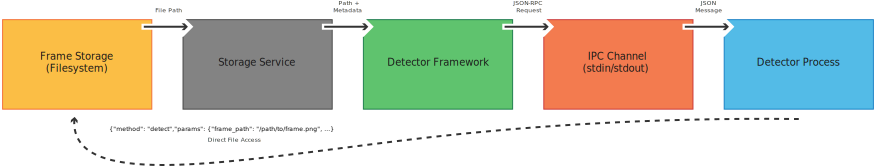
\includegraphics[width=0.8\textwidth]{figures/comms flow.png}
\caption{Communication flow between framework and sandboxed detectors. JSON-RPC messages contain frame paths rather than image data, reducing serialisation overhead whilst maintaining security through process isolation.}
\label{fig:comms-flow}
\end{figure} 
\subsection{Reliability Practices}
During the workload of monitoring anomalies, the key long-term component is consistent frame capture. CAM-F prioritises operational continuity through sophisticated failure handling that keeps it running regardless of various failures. The capture service operates independently from detector processing. Frames are queued asynchronously for detection, ensuring capture continues uninterrupted even during complete detector failures. Detector failures trigger progressive recovery through five strategies:
Immediate restart for transient failures
Exponential backoff (1-60 seconds) for recurring issues
Frame skipping for consistently problematic frames
Fallback mode with reduced processing quality
Automatic disabling after excessive consecutive failures
The recovery manager analyses failure patterns including consecutive failures, time-based clustering and frame-specific issues used in appropriate strategy selection. Recovery state persists to \texttt{detector\_recovery\_state.json}, preserving learned failure patterns across system restarts.
\section{Detector Design}
The detector architecture defines how individual detection algorithms integrate with CAM-F. Each detector operates as a self-contained unit that analyses frame pairs for specific continuity errors. This modular design allows researchers to develop specialised detectors without understanding the framework's internal complexity.
\subsection{Manifest Driven Architecture}
Every detector includes a \texttt{detector.json} manifest file that declares its capabilities and requirements. This manifest specifies whether the detector needs GPU access, how much memory it requires, and what configuration options users can adjust. The framework reads these declarations before running any detector code, preventing incompatible detectors from installing on systems that cannot support them. Configuration schemas automatically generate user interfaces, eliminating manual UI development. A few of the other configurations are there solely for inspiration and showcase of potential use-case scenarios. For example, memory declarations can allow the system to calculate whether multiple detectors can run simultaneously or not, notifying the user of computational limitations.
This design differs from traditional plugin systems that discover capabilities at runtime. By requiring explicit declarations, CAM-F provides transparency about resource usage. Script supervisors can understand why certain detectors need specific hardware or take longer to process frames. The manifest becomes a clear specification of what each detector does and what it needs to function.
\subsection{Three-Phase Execution Model}
Detectors follow three distinct phases: initialization, processing, and cleanup. This structure reflects common patterns in computer vision workflows where model loading represents a significant one-time cost.
During initialization, detectors load neural network weights and allocate GPU memory. This phase runs once when a detector activates, with costs amortised across thousands of subsequent frames. The framework enforces a configurable timeout (default 30 seconds) to prevent stuck detectors from blocking the system.
The processing phase handles frame pair analysis. Each invocation receives current and reference frames as NumPy arrays, along with metadata about take numbers and timestamps. Detectors analyse these inputs and return a list of detected errors. While the architecture encourages stateless processing for deterministic results, detectors can maintain internal state within their container lifetime if needed.
Cleanup ensures proper resource release when detectors deactivate. GPU memory must be freed and temporary files deleted. The framework monitors this phase with a configurable timeout, forcibly terminating detectors that fail to clean up properly.
\subsection{Error Reporting Structure}
Detector outputs follow a standardised format designed for production use. Each error report includes five components:
Error type: A categorical classification like \texttt{"prop\_missing"} or \texttt{"wardrobe\_change"} that enables filtering and statistical analysis.
Confidence score: A probability between 0.0 and 1.0 indicating detection certainty. Productions can adjust thresholds based on their tolerance for false positives.
Spatial location: A bounding box with x, y, width, and height coordinates for visual overlay on frames.
Description: Plain language explanation written for script supervisors, not engineers.
Details: Additional structured data like object classes or colour values for further processing.
This format is based on how script supervisors process information during production. Technical metrics alone are insufficient when they need to make rapid decisions. The combination of visual location, confidence score, and human-readable description provides the context needed for quick assessment.
\subsection{Communication Protocol}
The framework communicates with detectors through standard input and output streams using JSON-RPC messages. Each detector runs as a separate process, receiving commands through \texttt{stdin} and sending results through \texttt{stdout}. This approach provides real-time communication without the delays inherent in filesystem-based message passing. The choice of \texttt{stdin}/\texttt{stdout} ensures any programming language can create a detector by simply reading and writing text streams.
The protocol separates control messages from frame data to maintain efficiency. JSON messages contain only commands and metadata, while actual frames remain in filesystem storage. When the framework needs a detector to analyse frames, it sends paths rather than image data. This design keeps messages small and allows the operating system to handle efficient file access through memory mapping. A configurable timeout on each message exchange prevents failed detectors from blocking the entire system.

Python's multiprocessing queues manage the underlying communication complexity. Rather than implementing custom inter-process communication, the framework uses proven standard library components. This reduces potential bugs and simplifies maintenance whilst providing reliable message delivery between the framework and detector processes. The architecture trades a small amount of theoretical performance for substantial improvements in stability and overall comprehension.
\subsection{Development Experience}
The framework provides a \texttt{BaseDetector} class that abstracts away all communication and protocol complexity. Developers inherit from this class and implement only the detection logic, typically just adjusting the \texttt{process\_frame\_pair} method. The base class handles JSON-RPC parsing, timeout management, frame loading, and error serialisation automatically. This abstraction transforms what could be a complex distributed system into a simple Python class with minimal boilerplate.
Testing detectors locally requires no Docker installation. The framework supports dual-mode execution where detectors run as standard Python processes during development. Virtual environments provide dependency isolation without container overhead. Developers can attach debuggers, inspect variables, and iterate quickly on their algorithms. When ready for deployment, the same code runs in Docker containers without modification. This flexibility recognises that forcing containerisation during development would significantly slow the refinement.
The standardised project structure simplifies packaging and distribution. A detector requires only three files: the Python implementation, \texttt{requirements.txt} for dependencies, and the manifest. Developers package these as a ZIP archive for distribution. The framework handles all complexity of building Docker images, installing dependencies, and registering detectors. This minimal structure allows computer vision researchers to share their work without learning containerisation, package management, or deployment procedures.
\section{Production Workflow Integration}
Standalone System: CAM-F operates independently alongside script supervisors' current workflow rather than replacing established practices. It avoids the complexity of integrating with ScriptE, MovieSlate, and other proprietary studio systems. Each of these tools stores data differently and updates frequently. To mitigate added overhead of managing another system CAM-F produces universal formats for the outputs that work with any production workflow.
Hierarchical Export System: The export architecture allows reports at any production level. A take export contains just that take's errors and annotations. Scene exports include all takes organised by camera angles, while project exports encompass the entire production hierarchy. This granular control enables efficient knowledge distribution across departments. Script supervisors might export individual takes for immediate review, while post-production coordinators need complete scene documentation.
Automatic Reference Take Management: The first successful take at each camera angle becomes the continuity baseline, matching standard production practice. Subsequent takes compare against this reference automatically. Supervisors can override the selection if needed.
Scene-Based Configuration: Detector settings apply uniformly at the scene level. All angles and takes within a scene share the same configuration, reflecting how productions maintain consistent continuity standards throughout related shots. A car chase scene enables motion-based detectors while a dialogue scene prioritises prop and wardrobe checks. This flat configuration model eliminates complexity while serving most production needs.